\documentclass[conference]{IEEEtran}
\IEEEoverridecommandlockouts
% The preceding line is only needed to identify funding in the first footnote. If that is unneeded, please comment it out.
\usepackage{cite}
\usepackage{amsmath,amssymb,amsfonts}
\usepackage{algorithmic}
\usepackage{graphicx}
\usepackage{textcomp}
\usepackage{xcolor}
\def\BibTeX{{\rm B\kern-.05em{\sc i\kern-.025em b}\kern-.08em
    T\kern-.1667em\lower.7ex\hbox{E}\kern-.125emX}}

%additional packages
%\usepackage[ngerman]{babel}
\usepackage[utf8]{inputenc} 
\usepackage{hyperref} 
\usepackage{url}   
%%fuer abkuerzungen begin
\usepackage[acronym,hyperfirst = false]{glossaries}
\glsdisablehyper
%\usepackage[acronym,acronymlists={main, abbreviationlist},shortcuts,toc,description,footnote]{glossaries}
\newglossary[clg]{abbreviationlist}{cyi}{cyg}{List of Abbreviations}
\newglossary[slg]{symbolslist}{syi}{syg}{Symbols}
\renewcommand{\firstacronymfont}[1]{\emph{#1}}
\renewcommand*{\glspostdescription}{}	% Punkt am Ende jeder Beschreibung entfernen
\renewcommand*{\acrnameformat}[2]{#2 (\acronymfont{#1})}	% Langform der Akronyme
\makeglossaries
\date{\today}
\newacronym[description={Interface provided by an application or software to be able to implement other programs that uses the software as foundation.}]{API}{API}{Application Programming Interface}

\newacronym[description={In German ``Bundesministerium f\"ur Bildung und Forschung'' is a federal ministry among other things responsible for research projects and the education inside of Germany.}]{BMBF}{BMBF}{Federal Ministry of Education and Research}

\newacronym[description={Hardware component which allows external devices to transfer data directly into or from the memory without using the processor.}]{DMA}{DMA}{Direct Memory Access}

\newacronym[description={Method for storing a number of data items inside of a buffer. Elements which have been stored first will be read first as well.}]{FIFO}{FIFO}{First In, First Out}

\newacronym{FM}{FM}{Frequency Modulation}

\newacronym[description={Stateful network protocol for transfering files from one system to an other system in ``plaintext'' format. FTP requires a reliable, error correcting base protocol like the \gls{TCP}. Besides the ability to read and write files to/from a host, the FTP provides further functionalities like user authorization, directory listing, renaming, or alteration of file access permissions.}]{FTP}{FTP}{File Transfer Protocol}

\newacronym[description={Stateless network protocol built on top of a reliable transport protocol like \gls{TCP} for transfering data from one host to another one. HTTP is the mainly used protocol for web browser interactions with a web server.}]{HTTP}{HTTP}{Hypertext Transfer Protocol}

\newacronym[description={International council responsible for the development and administration of norms in the area of electrical engineering and electronics. Some standards are developed together with the \gls{ISO}.}]{IEC}{IEC}{International Electrotechnical Commission}

\newacronym[description={Primary used communication protocol (in the Internet) for transmitting data packets (or datagrams) from one system to another one. This protocol is located on the Internet layer of the \gls{OSI} and can be split into the older version IPv4 and the newer one IPv6 that allows to address more devices. (cf.\,\cite{Tanenbaum2003})}]{IP}{IP}{Internet Protocol}

\newacronym[description={Set of methods for exchanging data between various threads within a system. In this thesis the term does not include the communication between various physical devices connected via a network to each other.}]{IPC}{IPC}{Inter--Process Communication}

\newacronym[description={International council responsible for the development and administration of norms except in the scope of electrical engineering and electronics. Responsible for these areas is the \gls{IEC}.}]{ISO}{ISO}{International Organization for Standardization}

\newacronym[description={Short function or method that is called as soon as a (specific) interrupt hits the processor core.}]{ISR}{ISR}{Interrupt Service Routine}

\newacronym[description={\ldots}]{MISD}{MISD}{Multi Instruction, Single Data}

\newacronym[description={\ldots}]{MIMD}{MIMD}{Multi Instruction, Multiple Data}

\newacronym[description={The OSI is a design model describing the network stack in seven layers: 1. Physical Layer, 2. Data Link Layer, 3. Network Layer, 4. Transport Layer, 5. Session Layer, 6. Presentation Layer, and 7. Application Layer (sorted from lowest to highest). (cf.\,\cite{Tanenbaum2003}))}]{OSI}{OSI}{Open Systems Interconnection Reference Model}

\newacronym[description={Processor design strategy based on the usage of a little amount of simplified instructions to improve execution performance.}]{RISC}{RISC}{Reduced Instruction Set Computer/Computing}

\newacronym[description={\ldots}]{CISC}{CISC}{Complex Instruction Set Computer/Computing}

\newacronym[description={\ldots}]{SISD}{SISD}{Single Instruction, Single Data}

\newacronym[description={\ldots}]{SIMD}{SIMD}{Single Instruction, Multiple Data}

\newacronym[description={Communication protocol located on the transport layer of the \gls{OSI} that provides a reliable transfer of network packets, i.e. ordered delivery of a byte stream from one program to another one.  The connection between both communication partners is built by a handshaking mechanism. In TCP each received packet is receipted by the recipient. (cf.\,\cite{Tanenbaum2003})}]{TCP}{TCP}{Transmission Control Protocol}

\newacronym[description={Rudimentary version of \gls{FTP} that is built on top of \gls{UDP}. The TFTP implements just the basics of file transfer like read and write. User authorization or directory listing is not provided. Because the protocol is built on top of an unreliable transport protocol a simple packet acknowledgment and checksum verification is used for error correction.}]{TFTP}{TFTP}{Trivial File Transfer Protocol}

\newacronym[description={Communication protocol located on the transport layer of the \gls{OSI} that provides a simple transmission model for packets without the overhead introduced by mechanisms for providing reliability, ordering, or data integrity, like handshaking dialogues. In \gls{UDP} the error detection and error correction is outsourced to higher layers like the application itself. Thus it is assumed that errors either have no influence for successfully processing the use--cases, or the correction is implemented inside of the application's using protocols. (cf.\,\cite{Tanenbaum2003})}]{UDP}{UDP}{User Datagram Protocol}

\newacronym[description={\ldots}]{WCET}{WCET}{Worst Case Execution Time}

\newacronym[description={Text--based data format for application independent and platform independent exchange of information.}]{XML}{XML}{Extensible Markup Language}

\newacronym[plural=ISAs, firstplural=Instruction Set Architectures (ISAs)]{ISA}{ISA}{Instruction Set Architecture}

\newacronym[plural=CPUs, firstplural=Central Processing Units (CPUs)]{CPU}{CPU}{Central Processing Unit}

\newacronym{AES}{AES}{Advanced Encryption Standard}

\newacronym[plural=FPGAs, firstplural=Field-programmable Gate Arrays (FPGAs)]{FPGA}{FPGA}{Field-programmable Gate Array}
%%fuer abkuerzungen end 

        
\begin{document}

\title{Paper Title *TODO edit*}

\author{\IEEEauthorblockN{1\textsuperscript{st} Given Name Surname}
\IEEEauthorblockA{\textit{Faculity of Computer Science and Mathematics} \\
\textit{OTH Regensburg}\\
Regensburg, Germany \\
name.surname@st.oth-regensburg.de}
%\and
%\IEEEauthorblockN{2\textsuperscript{nd} Given Name Surname}
%\IEEEauthorblockA{\textit{dept. name of organization (of Aff.)} \\
%\textit{name of organization (of Aff.)}\\
%City, Country \\
%email address}
%\and
%\IEEEauthorblockN{3\textsuperscript{rd} Given Name Surname}
%\IEEEauthorblockA{\textit{dept. name of organization (of Aff.)} \\
%\textit{name of organization (of Aff.)}\\
%City, Country \\
%email address}
%\and
%\IEEEauthorblockN{4\textsuperscript{th} Given Name Surname}
%\IEEEauthorblockA{\textit{dept. name of organization (of Aff.)} \\
%\textit{name of organization (of Aff.)}\\
%City, Country \\
%email address}
%\and
%\IEEEauthorblockN{5\textsuperscript{th} Given Name Surname}
%\IEEEauthorblockA{\textit{dept. name of organization (of Aff.)} \\
%\textit{name of organization (of Aff.)}\\
%City, Country \\
%email address}
%\and
%\IEEEauthorblockN{6\textsuperscript{th} Given Name Surname}
%\IEEEauthorblockA{\textit{dept. name of organization (of Aff.)} \\
%\textit{name of organization (of Aff.)}\\
%City, Country \\
%email address}
}

\maketitle

\begin{abstract}
text
\end{abstract}

\begin{IEEEkeywords}
keyword1, keyowrd2
\end{IEEEkeywords}



\section{Introduction}
\label{ref:introduction}
text

\section{Background}
\label{ref:background}
text

\section{Related Work}
\label{ref:relatedwork}
text

\section{Concept and Methods}
\label{ref:concept}
text
 
\section{Implementation}
\label{ref:implementation}
text

\section{Evaluation}
\label{ref:evaluation}
text

\section{Discussion}
\label{ref:discussion}
text

\section{Concusion and Outlook}
\label{ref:conclusion}
text

% ----------------------------------------------------------------------------------
% Kleine Einführung in LaTeX-Elemente
% ----------------------------------------------------------------------------------
\section*{Tipps für Latex}
Dieser Abschnitt beinhaltet lediglich einige Informationen über \LaTeX-Distributionen, Editoren und \LaTeX-Elemente, die Ihnen beim Einstieg in das \LaTeX-Textsatzsystem helfen sollen.

\subsection{\LaTeX-Distributionen nach Betriebssystemen}

\subsubsection{\LaTeX-Distributionen}
Folgende Haupt-\LaTeX-Distributionen stehen Ihnen zur Verfügung:
\begin{itemize}
  \item Windows:\quad \texttt{ProText}\quad Webseite:\quad\url{https://www.tug.org/protext/}    
  \item Windows:\quad \texttt{MiKTeX}\quad Webseite:\quad\url{http://www.miktex.org}
  \item Linux/Unix:\quad \texttt{TeX Live}\quad Webseite:\quad\url{http://tug.org/texlive/}
  \item Mac OS:\quad \texttt{MacTeX}\quad Webseite:\quad\url{http://www.tug.org/mactex/}
\end{itemize}
Empfehlung: Nehmen Sie ProText und installieren Sie es in der Vollinstallation. ProText ist eine Art 'fullbundle' von MiKTeX. Die Vollinstallation ist zwar etwas groß und dauert etwas, aber dafür gibt es kein Problem mit evtl fehlenden Paketen.
Diese Vorlage wurde getestet mit folgendender Version:
ProTeXt-3.1.9-121317.exe \\ 
\url{http://ftp.math.utah.edu/pub/tex/historic/systems/protext/2018-3.1.9/} \\
Diese Version befindet sich auch auf dem Laufwerk der Labor-PCs:\\
\verb|L:\DT\Professoren\Muench\tools| \\  
Oder unter folgendem Link befinden (wenn Sie sich über VPN einwählen): \\
\verb|\\rfhinffs1.hs-regensburg.de\labor\DT|\\ \verb|\Professoren\Muench\tools|\\
Verwenden Sie bei Problemen die oben genannte Version.

\subsubsection{\LaTeX-Editoren}
Auf folgenden Webseiten können Sie einige hilfreiche \LaTeX-Editoren finden:
\begin{itemize}
  \item Windows/Linux/Mac OS: \url{http://www.xm1math.net/texmaker/}
  \item Windiws: \url{http://www.texniccenter.org/}
  \item Mac OS: \url{http://pages.uoregon.edu/koch/texshop/}
\end{itemize}

Falls bei den oben genannten Editoren kein passender vorhanden war, findet sich auf Wikipedia eine Zusammenstellung vieler weiterer \LaTeX-Editoren:\\
\url{https://en.wikipedia.org/wiki/Comparison_of_TeX_editors}

Für die PDF-Anzeige empfiehlt sich SumatraPDF: \\ 
\url{https://www.sumatrapdfreader.org/free-pdf-reader.html}. \\
Empfehlung: SumatraPDF lockt die Datei nicht wie die meister PDF-Reader. Somit können sich kontinuierliche Updates machen und müssen die PDF-Datei nicht immer schließen und wieder öffen.



\subsection{Bilder}
Zum Einfügen eines Bildes, siehe Fig. \ref{fig:reversi01}, wird  der Befehl \texttt{$\backslash$includegraphics} genutzt.

\begin{figure}[htbp]
	\centering
	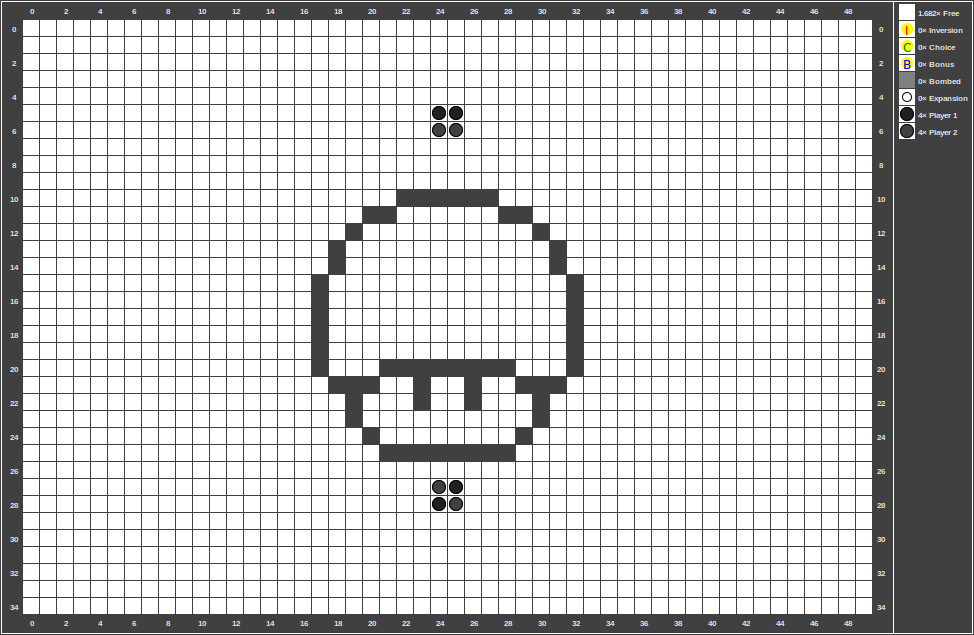
\includegraphics[width=0.7\linewidth]{figures/gamefield01.png}
	\caption[Spielfeld 01]{Unbespieltes Spielfeld}
	\label{fig:reversi01}
\end{figure}

Nachdem das Spielt gestartet wurde und beide Spielphasen durchlaufen wurden, siegt schließlich der Spieler mit der Farbe rot. Fig. \ref{fig:reversi02} zeigt ...

\begin{figure}[htbp]
	\centering
	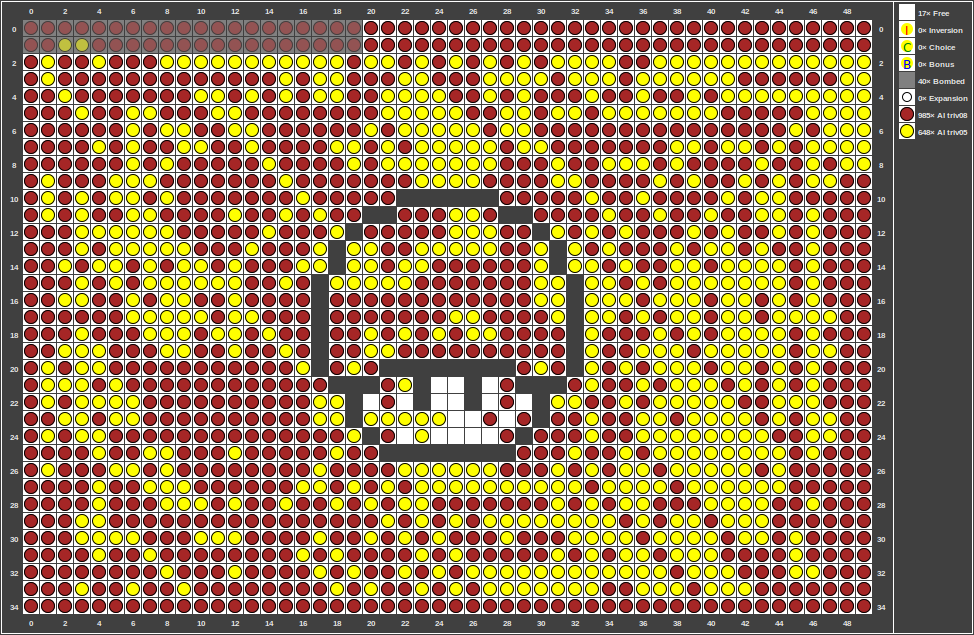
\includegraphics[width=0.7\linewidth]{figures/gamefield02.png}
	\caption[Spielfeld 02]{Finales Spielfeld}
	\label{fig:reversi02}
\end{figure}


\subsection{Tabellen}
In diesem Abschnitt wird eine Tabelle (siehe Tabelle \ref{tab:beispiel}) dargestellt.

\begin{table}[!h]
	\centering
  \caption{Beispieltabelle}
	\label{tab:beispiel}
	\begin{tabular}{|l|l|l|}
		\hline
		\textbf{Name} & \textbf{Name} & \textbf{Name}\\
		\hline
		1 & 2 & 3\\
		\hline
		4 & 5 & 6\\
		\hline
		7 & 8 & 9\\
		\hline
	\end{tabular}	
\end{table}


\subsection{Auflistung}
Für Auflistungen wird die \texttt{enumerate}- oder \texttt{itemize}-Umgebung genutzt.

\begin{itemize}
	\item Nur
	\item ein
	\item Beispiel.
\end{itemize}


\subsection{Gleichungen}
Formatierung von Formeln:

\begin{itemize}
  \item Formelzeichen sind in kursiv zu setzen
  \item Zahlen, Einheiten und Funktionsnamen sind in normaler Schriftart zu setzen (nicht kursiv)
  \item Häufig wird fälschlicherweise das Symbol * als Multiplikationszeichen verwendet
  \item Zwischen Zahl und Einheit ist ein Leerzeichen zu setzen
\end{itemize}

\gls{FM} is a wireless transmission system patent-registered by Edwin H. Armstrong in 1933. It is still widespread in the area of audio broadcasting today. In case of the frequency modulation the amplitude of the desired message signal varies the frequency (the argument) of the sinusoidal carrier. The general \gls{FM} oscillation is formulated with 
\begin{equation}
u_{\textrm{FM}}(t)= a_0 \cos(\Psi(t)+\varphi_0) 
\label{eqn:fmosc}
\end{equation}

To simplify matters, only an one-tone modulation signal is considered to characterize the spectrum of \gls{FM} -signals at first
\begin{multline}
u_{\textrm{FM}}(t)=\hat u_T \cdot [J_0(\eta)\cos\omega_Tt +
\\ \sum_{n=1}^{+\infty} J_n(\eta) \cdot (\cos[(\omega_T+n\omega_1)t]+
\\(-1)^n \cos[(\omega_T-n\omega_1)t])] 
\\ \ \mbox{with Bessel functions:} 
\\ \ J_n(\eta)= \frac{(-1)^n}{\pi} \int_0^{\pi} e^{j\eta\sin x} \cdot \cos(nx) dx 
\end{multline}

\subsection{Verwendung von Abkürzungen}
Die Abkürzungen werden in glossary.tex definiert. Die Abkürzungen können so verwendet werden:
Beim ersten Mal der Verwendung wird die Abkürzung ausgeschrieben z.B. \gls{TCP}. Beim zweiten Mal oder folgenden Malen wird nur noch die Abkürzung verwendet z.B. \gls{TCP}.
Aber setzen Sie Abkürzungen sparsam ein.

\subsection{Literaturverzeichnis}
Die Quellen befinden sich in der Datei \textit{biblography.bib}. 
Alle Literaturangaben müssen im Text referenziert werden. Die höchstwertigen Quellen stellen dabei Zeitschriftenartikel \cite{Laprie2004}, gefolgt von Konferenzbeiträgen \cite{Agrou2011}, Patenten \cite{Grisenthwaite2012}, Standards \cite{ARINC2005}, Fachbüchern \cite{Kopetz2011},  Datenblättern \cite{Freescale2015}, Techreports und White-Papern \cite{Aswadhati2011} und zuletzt Onlinequellen \cite{Xil2010} dar.

\bibliographystyle{IEEEtran}
\bibliography{bibliography}

\end{document}
